\documentclass[10pt]{article}
\usepackage[utf8]{inputenc}
\usepackage[margin=1in]{geometry}
\usepackage{array}
\usepackage[]{hyperref} 
\hypersetup{
    colorlinks,
    linkcolor={red!50!black},
    citecolor={blue!50!black},
    urlcolor={blue!80!black}
}

\usepackage[]{mathtools} 

\usepackage[]{graphicx} 
\usepackage[]{tikz} 
\usepackage[]{xcolor} 

\usepackage[]{tab} 


\title{Spreadsheets for Physics Labs}
\author{University of Minnesota Teaching Assistants, 2020}
\def\Subtitle{Sheets}
\date{\today}
\makeatletter
\let\Date\@date
\let\Author\@author
\let\Title\@title
\makeatother

\usepackage{fancyhdr}
\pagestyle{fancy}
\lhead{\Title}
\rhead{\leftmark}
\rfoot{Page \thepage}\lfoot{}\cfoot{}
\fancypagestyle{plain}{%
  \fancyhf{}%
  \renewcommand{\headrulewidth}{0pt}
    \fancyfoot[R]{Page \thepage}%
}



\usepackage{tcolorbox}
\tcbuselibrary{theorems}
\newtcolorbox{exercise}{
    enlarge top initially by=2mm,
    enlarge bottom finally by=2mm,
    arc=3pt,
    boxrule=1pt,
    colframe=red!50!black,
    colback= red!5,
    fonttitle=\bfseries,
    title=Exercise
}
\newtcolorbox[auto counter, number within=section]{keyinfo}[2]{
    enlarge top initially by=2mm,
    enlarge bottom finally by=2mm,
    arc=3pt,
    boxrule=1pt,
    colframe=green!50!black,
    colback= green!5,
    fonttitle=\bfseries,
    title=Core Idea \thetcbcounter: #1,
    label=key:#2
}
\newtcolorbox[auto counter, number within=section]{example}[2]{
    enlarge top initially by=2mm,
    enlarge bottom finally by=2mm,
    arc=3pt,
    boxrule=1pt,
    colframe=blue!80!black!90!,
    colback= blue!5,
    fonttitle=\bfseries,
    title=Example \thetcbcounter: #1,
    label=ex:#2
}
\newtcolorbox[auto counter, number within=section]{summarybox}[1]{
    arc=0pt,
    boxrule=1pt,
    colframe=black!80,
    colback= white,
    fonttitle=\bfseries,
    title=#1, 
}





\begin{document}
\begin{center}
    \thispagestyle{empty}
    \vspace*{3cm}
    {\bfseries\Huge \Title}\\
    \vspace{0.5cm}
    {\huge \Subtitle}\\

	\vspace{1cm}
		\centering
		
\includegraphics[width=0.8\linewidth]{images/excel.jpg}

    \vspace{2cm}
    {\Author}\\\vspace{1cm}
    {Last Update: \Date}
\end{center}
\newpage
\tableofcontents
\newpage

\newenvironment{sheetpic}{\begin{center}\begin{tikzpicture}}{\end{tikzpicture}\end{center}}

\def\annotateIm#1#2#3#4#5#6{\path #1 ++ (#2:#3) node[#5] (temp) {#4};\draw[-latex,#6] (temp) -- #1;}

\section{Introduction}%
\label{sec:introduction}

Spreadsheet programs are a basic tool for getting started with data analysis. 
The following information should be enough to get you started on using spreadsheets and give you enough knowledge to let  you complete (more or less) any task that gets thrown at you in introductory labs. 


\subsection{List of Spreadsheet Software}%
\label{sub:listof}

There are a number of different spreadsheet programs, but, fortunately, their core functionality is very similar. 
Below is a list of some of the major options available for to you:

\begin{description}
    \item[Microsoft Excel] The big one. This is the program we will be assuming you are using, though most other spreadsheet programs emulate it. 
        It is paid software, but UMN students can access it for free at \href{https://it.umn.edu/services-technologies/how-tos/microsoft-office-365-pro-plus-faculty}{via the UMN website}.
    \item[Google Sheets] The premier online spreadsheet program. Anyone can access it through their google account. Its functionality is more limited than Excel and it is slower, but is still fully capable of doing the required analysis.
    \item[LibreOffice Calc] The open source alternative to Excel, the libre office suite is good for those who can't access Excel but still want a reasonbly powerful spreadsheet program to run locally on their computer.
		It can be downloaded for free from the \href{https://www.libreoffice.org/discover/calc/}{LibreOffice website}.
\end{description}


\begin{exercise}
	Download (or just navigate to) one these programs. 
\end{exercise}



\newpage

\section{The Basics of Spreadsheets}%
\label{sec:the_basics_of_spreadsheets}

In this section we will quickly review the basics of spreadsheet programs.
By the end of this section you should understand 
\begin{itemize}
	\item How cells are labeled.
	\item How to enter values into cells and how to control their formatting.
	\item How to write formulas, and how to use other cells as inputs in formulas.
\end{itemize}


\subsection{The layout of the spreadsheet}%
\label{sub:the_layout_of_the_spreadsheet}


A spreadsheet is a collection of cells, arranged into rows and columns. 
The column of the cell is indexed by letters A, B, C, \ldots\ and the rows are labeled by numbers 1, 2, 3, \ldots\ . 
The appearence of a general spreadsheet is shown in Fig.~\ref{fig:blank_sheet}. 
\begin{figure}[htpb]
	\centering
	\begin{sheetpic}
		\etab[3]{A-D}
		\node (X) at (1,1) {Each of these squares is a cell.};
		\draw[latex-] (cellA-2.center) -- (X);
		\draw[latex-] (cellD-3.center) -- (X);
		\draw[latex-] (cellB-1.center) -- (X);
		\annotateIm{(cellB-2.center)}{-60}{2}{This is cell B2}{}{}
	\end{sheetpic}
	\caption{A basic spreadsheet.}%
	\label{fig:blank_sheet}
\end{figure}

%\begin{figure}
%\begin{sheetpic}
%    \etab[5]{A-F}
%    \annotateIm{(cellA-3.center)}{60}{3}{A cell in a spreadsheet}{draw}{thick}
%    \celtxt{C}{3}{Some text}
%    \celtxt{D}{2}{=B1^2 - 3}
%    \annotateIm{(cellD-2)}{-120}{3}{Cells can contain formulas \\ that reference other cells}{draw, align=center}{thick}
%    \fillCol{E}{2}{5}{\row*2}{c}
%    \celtxt[c]{F}{1}{E1^2-3}
%    \celtxt[c]{E}{1}{2}
%    \calcCol{F}{2}{5}{E}{\x ^ 2 - 3 }{c}
%    \annotateIm{(cellF-1)}{120}{2}{Cell forumlas can be propagated,\\ allowing you to quickly do calculations\\ on a large amount of data}{draw, align=center}{thick}
%\end{sheetpic}
%\caption{The basic layout of a spreadsheet program.}
%\label{fig:many_features}
%\end{figure}


To edit the contents of a cell simply double click on it, or click once to select it then just start typing. 
Let's talk briefly about what can go into a cell. 

\subsection{Values in a cells}%
\label{sub:values_in_a_cells}

There are, more or less, two types of values that can go in a cell. 
One is a \textit{formula} which we will discuss at length in Sec.~\ref{sec:formulas}. 
The other is a literal value, which we will discuss here. 
A literal value is just some value -- a number, a word, a date, etc. 

\begin{figure}[htpb]
	\centering
	\begin{sheetpic}
		\etab[3]{A-D}
		\celtxt[c]{A}{2}{A string}
		\celtxt[c]{B}{1}{123}
		\celtxt[c]{B}{2}{3124}
		\celtxt[c]{B}{3}{3.124e3}
	\end{sheetpic}
	\caption{Some examples of values in a cell. }%
	\label{fig:valsincells}
\end{figure}

A few examples are shown in Fig.~\ref{fig:valsincells}.
Notice that cells B2 and B3 contain the same value, just expressed in different ways (normal and scientific notation).
This is an instance of a more general process of formatting that occurs in spreadsheet programs.
You, the user, have control over both the value and how it appears within the program.
In Excel, this is controlled using the number menu which is shown on the far right in Fig.~\ref{fig:images_Menu}.

\begin{figure}[htpb]
	\centering
	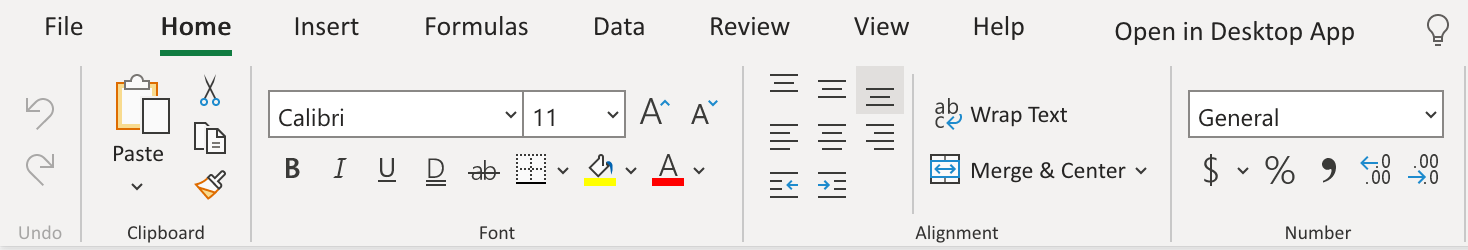
\includegraphics[width=0.8\linewidth]{images/Menu.png}
	\caption{The Excel menu. Observe the number section on the far right. }%
	\label{fig:images_Menu}
\end{figure}

You should make frequent use of this menu as you input data, as it allows you to express it in easier-to-read forms.
In particular, pay attention to the precision option, indicated by the \raisebox{-0.4em}{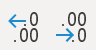
\includegraphics[height=1.5em]{images/prec.png}} button. 
These two buttons increase and decrease the precision of a number. 
Note that this does not change the number itself, only how it is displayed; behind the scenes Excel always has the full number. 

You should make use of the this feature extensively when making graphs, top avoid having unrealistic precisions in your labels. 

Spend a few minutes playing around with these options. Make sure you are able to change the precision and the notation. 

\subsection{Value Extrapolation}%
\label{sub:value_extrapolation}

One thing that remains to be seen is how we can fill out a large number of cells without entering values one by one. 
This is done through \textit{extrapolation}.
This process involves taking some number of ``base" cells, which contain some values (or formulas, as we will see later) and then ``dragging" them to cover a larger region.
In this process, the program will guess how to fill in the blank cells, often quite accurately.
An example of this is show in Fig.~\ref{fig:extrapolation}.


\begin{figure}[htpb]
	\centering
	\begin{minipage}{0.5\textwidth}
	\begin{sheetpic}
		\etab[10]{A-B}	
		\fillCol{A}{1}{3}{\row}{c}
		\multiSelec{A-1}{A-3}
		\annotateIm{($(cellA-3.south east)+(0.15,-0.15)$)}{-45}{3}{By dragging this small \\ square at the bottom  of a \\ selection region, you can \\ extrapolate the  values to the \\ area you drag it.}{fill=white,draw,align=center}{}
	\end{sheetpic}
	\end{minipage}
	\begin{minipage}{0.3\textwidth}
	\begin{sheetpic}
		\etab[10]{A-B}	
		\fillCol{A}{1}{10}{\row}{c}
		\multiSelec{A-1}{A-10}
	\end{sheetpic}
\end{minipage}
	\caption{
	An example of value extrapolation.
	We first fill in a few values, here 1,2, and 3 in cells A1, A2, and A3.
	By selecting the cells and then dragging the region to cover the cells A1-A10 we see that the program extrapolates the values -- it assumes we want to increment by 1 each time}%
	\label{fig:extrapolation}
\end{figure}

\begin{exercise}
	Can you figure out a way to fill a region with with the values $0.1,0.2, \ldots, 1$?
\end{exercise}



\section{Formulas}%
\label{sec:formulas}

As mentioned in Sec.~\ref{sub:values_in_a_cells} there are two types of things that can go in cells. 
We have discussed literal values, and we now we talk about the more interesting one: formulas. \textbf{To tell the cell that we want to use a formula, the first character in the cell must be the ``=" (the equal sign)}.
The remainder of the cell is the formula. 


\subsection{Basic Formula Syntax}%
\label{sub:basic_formula_syntax}


Once we have done this we can make use of all the normal mathemtical operations, as well as a large number of built-in functions.
Lets see how this works.
To add, substract, mutliply, or divide, we use the normal symbols: $+,-,*,$ and $/$.
Functions are always written in all capital letters.
For example, to take the Square Root of a number, we would enter it like: \texttt{SQRT(5)}. 

\begin{table}[htpb]
	\centering
	\begin{tabular}{c|>{\texttt}c}
	Mathematical function & Excel Name  \\\hline
	A $(+,-,*,/)$ B & A $(+,-,*,/)$ B \\
	$A^{B}$ & A \textasciicircum B \\
	
	$\sqrt{A}$ & SQRT(A) \\
	$\ln{A}$ & LOG(A) \\
	$\sin \left( A \right)$ &  SIN(A) \\
	$\cos \left( A \right)$ &  COS(A) \\
	$\tan \left( A \right)$ &  TAN(A) \\
	$\sin^{-1} \left( A \right)$ (and co.) &  ARCSIN(A) \\
	\end{tabular}
	\caption{Common functions and their names}
	\label{tab:funcs}
\end{table}


Table~\ref{tab:funcs} should describe all the functions you will need in the course.
However, if you find yourself needing some function not found here, normally a quick google for ``Excel how to  \ldots ", will tell you what you need.
An important note is that parentheses are also used to group elements (in addition to denoting the arguments of functions).
Make sure to use them to avoid order-of-operations errors. 

Lets translate some functions to Excel. 


\begin{table}[htpb]
	\def\x{$*$ }
	\centering
	\renewcommand\arraystretch{2}
	\begin{tabular}{c|>{\texttt}c}
	Mathemtical Expression & Equivalent Excel Formula  \\\hline
	$\displaystyle 4 \frac{\sin \left( 2 \pi\right)}{23 + 4}$ & = 4 \x SIN(2 \x PI) / ( 23 + 4)  \\
	$\displaystyle \left( 20 + 5.3 \right)^{ \frac{4}{3} }$& = ( 20 + 5.3) \textasciicircum\ ( 4 / 3)
	\end{tabular}
	\caption{Some math formulas and their Excel equivalents.}
	\label{tab:formulas}
\end{table}

\begin{exercise}
	Flip through your physics textbook or exam equation sheet.
	Try to translate some of the equations to Excel. 
\end{exercise}

\subsection{Variables}%
\label{sub:variables}

Of course, right now what we have shown is really no better than entering values manually.
The real strength of formulas is that we may use the values of other cells as variables in our formula.
Cells are denoted by their column and then their row.
For example : A3, B12, or C21 (like in the game battleship).
If we type in a cell name (or click on the cell) while entering a formula, then Excel will replace the cell with its value when it is evaluating the formula.

For example, suppose in cell C3 we entered the formula: \raisebox{0.3ex}{\fbox{ \texttt{= (A2 + B3)\textasciicircum\ 2}}}. 
Then the value of the cell C3 would be the square of the sum of the values of the cells A2 and B3. Note that if a cell is empty, it is normally treated as zero. Lets look at some more examples

\begin{figure}[htpb]
	\centering
\begin{minipage}{0.4\textwidth}
	\begin{sheetpic}
		\etab[5]{A-B}
		\celtxt[c]{A}{1}{3}
		\celtxt[c]{A}{2}{=A1 + 3}
		\celtxt[c]{B}{4}{=A2 ^ 2 + A1}
	\end{sheetpic}
\end{minipage}
\begin{minipage}{0.4\textwidth}
	\begin{sheetpic}
		\etab[5]{A-B}
		\celtxt[c]{A}{1}{3}
		\celtxt[c]{A}{2}{6}
		\celtxt[c]{B}{4}{39}
	\end{sheetpic}
\end{minipage}
	\caption{Examples of using formulas.
	The sheet on the left shows the formulas and the sheet on the right shows how it would appear to the user.
Notice that, as shown in cell B4, we can use cells containing formulas as variables in other formulas.
}%
	\label{fig:forumula_example_1}
\end{figure}

\subsection{Formula Extrapolation}%
\label{sub:formula_extrapolation}

Often we wish to fill in a large area with a formula.
Just like filling in values, this can be done with \textit{extrapolation}.
The key difference between formula extrapolation and value extrapolation is what is extrapolated.
In value extrapolation, as we saw, the program guessed at the values of the filled in cells and replaced the values. 

In formula extrapolation, what is extrapolated are the variables, and for good reason.
Normally we write formulas that reference values in the same row, so when we drag out the formulas, we still want them to reference the row in which they are found
	
\begin{figure}[htpb]
	\centering
\begin{minipage}{0.4\textwidth}
	\begin{sheetpic}
		\etab[5]{A-B}
		\fillCol{A}{1}{5}{\row}{c}
		\celtxt[c]{B}{1}{=1+A1^2}
		\selecCell{B}{1}
	\end{sheetpic}
\end{minipage}
\begin{minipage}{0.4\textwidth}
	\begin{sheetpic}
		\etab[5]{A-B}
		\fillCol{A}{1}{5}{\row}{c}
		\multiSelec{B-1}{B-5}
		\foreach \x in {1,...,5}{
		\celtxt[c]{B}{\x}{=4.9*A\x\textasciicircum2};
	}
	\end{sheetpic}
\end{minipage}
	\caption{Extrapolating a formula. Notice how each cell in column $B$ still references the row in which it is found.}%
	\label{fig:formula_extrapolation}
\end{figure}

Formula extrapolation will be one of your most used tools, so please spend some time playing with it. 

\subsubsection{Static Values}%
\label{ssub:static_values}

One final note is that sometimes you may not want your formula to extrapolate.
For example, say you write the value for one half the acceleration due to gravity (in m/s) $4.9$ in cell  C1, and then replaced the value $4.9$ in the left hand sheet in Fig.~\ref{fig:formula_extrapolation} with C1.
This works well, except when we extrapolate this value, the C1 value gets extrapolated as well! This can be solved by replacing C1 with \$C\$1.
The dollar signs tell the program that we do not want this value to be extrapolated. 
\begin{figure}[htpb]
	\centering
\begin{minipage}{0.4\textwidth}
	\begin{sheetpic}
		\etab[5]{A-B}
		\fillCol{A}{1}{5}{\row}{c}
		\multiSelec{B-1}{B-5}
		\foreach \x in {1,...,5}{
		\celtxt[c]{B}{\x}{=C\x*A\x\textasciicircum2};
	}
	\end{sheetpic}
\end{minipage}
\begin{minipage}{0.4\textwidth}
	\begin{sheetpic}
		\etab[5]{A-B}
		\fillCol{A}{1}{5}{\row}{c}
		\multiSelec{B-1}{B-5}
		\foreach \i in {1,...,5}{
		\celtxt[c]{B}{\i}{=\char"24 C\char"24 1*A\i\textasciicircum2};
	}
	\end{sheetpic}
\end{minipage}
	\caption{The use of static variables. }%
	\label{fig:static_vars}
\end{figure}



\section{Graphs}%
\label{sec:graphs}

We've now come to perhaps the most important part of the tutorial: graphs.
Graphs are the way you present your data in a lab report, and so it is important to understand how to use them effectively. 

Let's review the basics of how graphs work in most spreadsheet programs.
A graph has a style.
This descibes its general form.
If you navigate to the ``insert'' tab in the top bar of Excel, you'll see several buttons corresponding to different chart styles:

\begin{figure}[htpb]
	\centering
	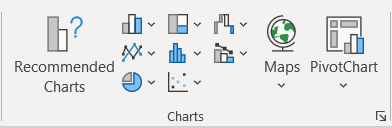
\includegraphics[width=0.6\linewidth]{images/chart-style.png}
	\caption{Different chart styles available in Excel}%
	\label{fig:images_chart-style}
\end{figure}

Though Excel and friends contain an enormous array of different graph styles, you will almost always use the \textit{scatter plot} graph style.
Note that, stylistically, you should plot your data as separate \textit{points} rather than as being connected by lines.

To actually insert such a plot, select the ``insert'' tab like before, then click the chart which looks like a scatter plot.
A drop down menu will appear with several different scatter plot variations.
Typically you will want to use the one with points which are \textit{not} connected by lines.

\begin{figure}[htpb]
	\centering
	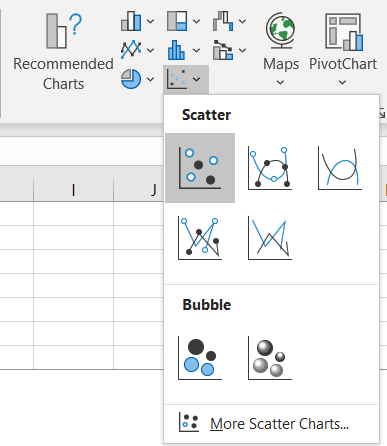
\includegraphics[width=0.3\linewidth]{images/insert-scatter-plot.png}
	\caption{Inserting a scatter plot into Excel}%
	\label{fig:images_insert-scatter-plot}
\end{figure}


Excel has two menus dedicated to the modification of a chart.
When you select a chart by clicking on it, two new tabs will appear in the ribbon: \textit{Chart Design} and \textit{Format}.
These two tabs provide the commands to modify the chart's data and style.

\begin{figure}[htpb]
	\centering
	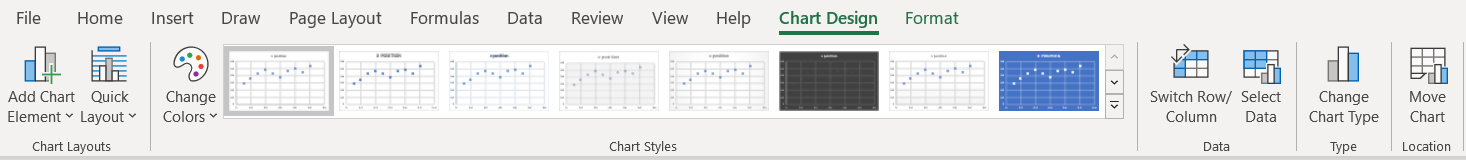
\includegraphics[width=1\linewidth]{images/chart-design-format.png}
	\caption{The \textit{Chart Design} and \textit{Format} tabs}%
	\label{fig:images_chart-design-format}
\end{figure}

This section will explain how you take the data from your sheet, plot it, and make it visually appealing.


\subsection{Adding Data to a Chart}%
\label{sub:adding_data_to_a_chart}

Each graph contains one or more \textit{data series}.
A data series is just a collection of $\left( x,y \right)$ values.
Often you will only need one data series, but sometimes you will want to plot several things at once, in which case you will use multiple data series.
If you have more than one data series, you must give each on a name so that the program can distinguish them.
In general then, you will also want to have a \textit{legend} so the reader of the graph can tell what data each set of points corresponds to. 

If you had some rows or columns selected when you inserted the chart into the document, the program will automatically assume that you want to plot those selected cells, and will create a data series containing this range of cells.
This can be unreliable, however. 

To accurately control the data in your chart, you can select your chart, use the ``select data'' option which is available in both the ``Chart Design'' tab, and the menu that comes up when you right click the scatter chart.
When you do this, the following chart in Fig.~\ref{fig:images_select-data}

\begin{figure}[htpb]
	\centering
	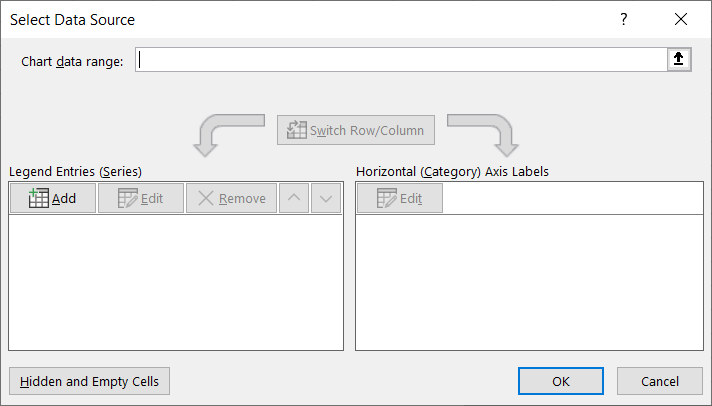
\includegraphics[width=0.5\linewidth]{images/select-data.png}
	\caption{The ``Select Data'' pop up window}%
	\label{fig:images_select-data}
\end{figure}

To add a data series, just click the ``Add'' button.
This brings up the window in Fig.~\ref{fig:images_data-series-selector}

\begin{figure}[htpb]
	\centering
	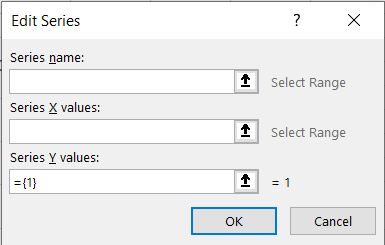
\includegraphics[width=0.5\linewidth]{images/data-series-selector.png}
	\caption{The pop up window which allows you to select your data series}%
	\label{fig:images_data-series-selector}
\end{figure}

First you must name your series.
To do this, either type a name into the ``Series name:'' box or click that box and select a cell which already contains a name.

To select the $x$-values for your data, click the ``Series X values:''  box and then click and drag on the spreadsheet to select the cells which contain your $x$-data.
\textit{Important}: make sure that the ``Series X values:'' box is empty before selecting your data cells.
The process for selecting your $y$-data is identical, except using the ``Series Y values:'' box.
You should end up with a scatter plot similar to in Fig.~\ref{fig:images_plain-chart}

\begin{figure}[htpb]
	\centering
	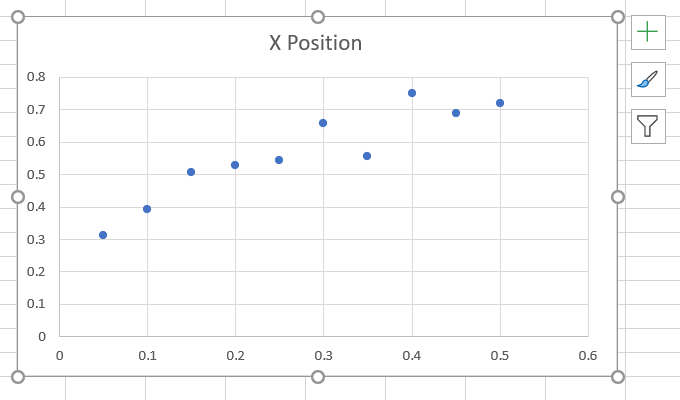
\includegraphics[width=0.8\linewidth]{images/plain-chart.png}
	\caption{A scatter plot after you've entered your data}%
	\label{fig:images_plain-chart}
\end{figure}

Adding a data series is identical.
To edit or remove an existing data series, select your data series in the pop-up window and press the ``Edit'' or ``Remove'' button respectively.

\subsection{Parts of the Charts}%
\label{sub:parts_of_the_charts}

To make your chart make sense to a reader, you need to add several other elements, including axis labels and a legend.
To add elements like these, click the ``+'' button in the top right corner of the plot -- this can be seen in Fig.\ref{fig:images_plain-chart}.
All of the parts of a chart are labeled in Fig.~\ref{fig:images_full-chart-labeled}. 

\begin{figure}[htpb]
	\centering
	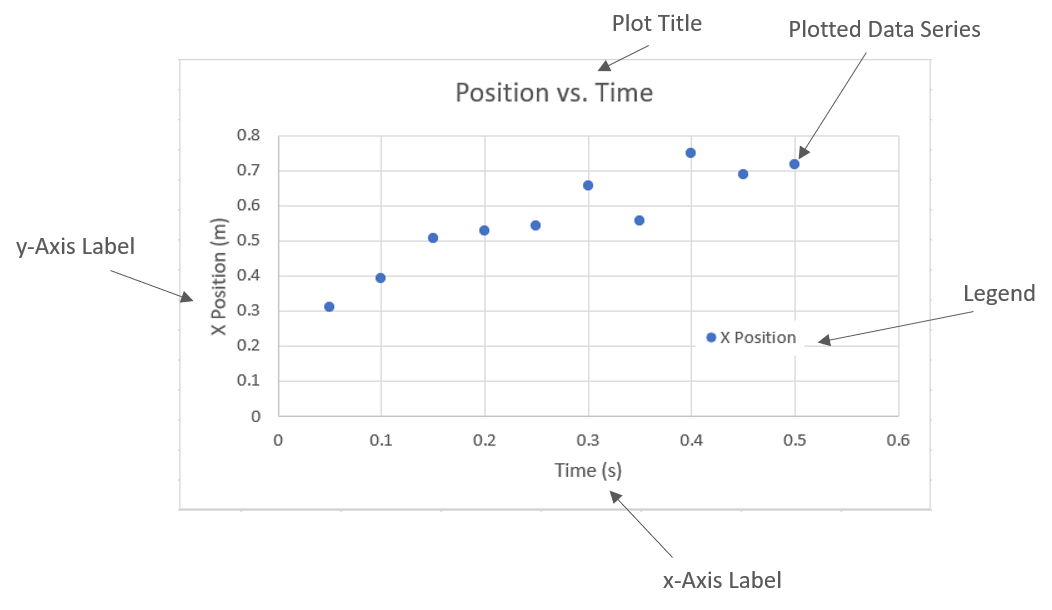
\includegraphics[width=0.8\linewidth]{images/full-chart-labeled.png}
	\caption{
		A chart with all of the parts labeled. 
		Note that the user can modify all of these parts.}%
	\label{fig:images_full-chart-labeled}
\end{figure}

%% \begin{figure}[htpb]
%% \begin{center}
%% \begin{tikzpicture}[scale=1, transform shape]
%% 	    \node[anchor=south west,inner sep=0] (image) at (0,0) {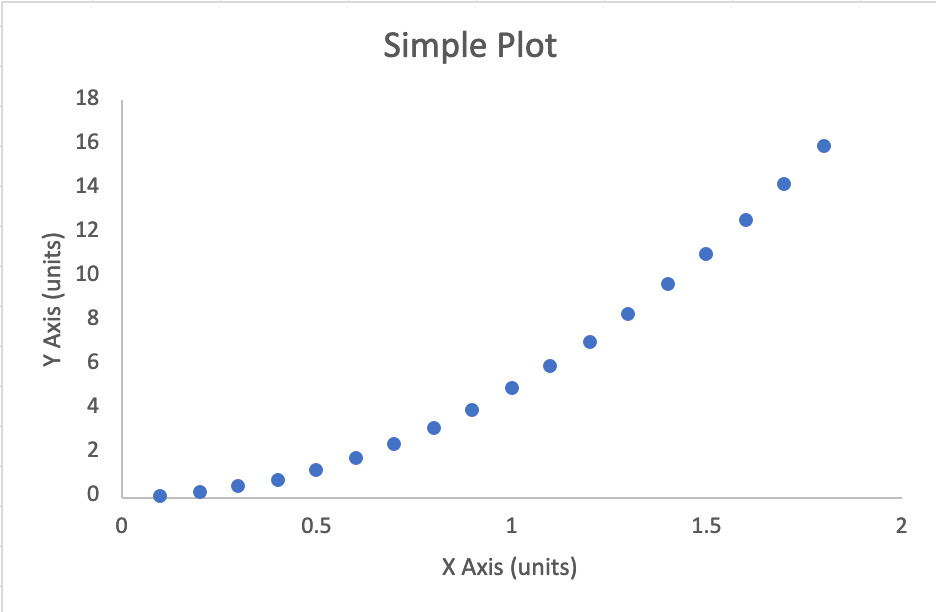
\includegraphics[width=0.7\textwidth]{images/simple_plot1.png}};
%%     \begin{scope}[x={(image.south east)},y={(image.north west)}]
%% 		\annotateIm{(0.55,0.05)}{-30}{0.2}{The x axis label}{}{}
%% 		\annotateIm{(0.55,0.95)}{30}{0.2}{The plot title}{}{}
%% 		\annotateIm{(0.03,0.5)}{140}{0.2}{The y axis label}{}{}
%% 		\annotateIm{(0.8,0.7)}{140}{0.1}{A plotted data series}{}{}
%%     \end{scope}
%% \end{tikzpicture}
%% \end{center}
%% \caption{A simple Excel plot. Every part can be changed by the user.}%
%% \label{fig:parts-of-chart}
%% \end{figure}
For the axis labels, make sure that you include \textit{units} -- here we have units of meters on the $y$-axis and units of seconds on the $x$-axis.
The legend displays all of the data markers (here a single blue circle) alongside the title of the data series.
Remember that you can change the name by using the ``Select Data'' function.
If you have multiple data series represented in the chart, you may choose which to show by clicking the funnel-looking thing below the paintbrush (see Fig.~\ref{fig:images_plain-chart}).
Also, you can change the formatting of the chart (including the size of the gridded area, location of the legend, location of the axis labels, etc.) by clicking around on the figure and dragging/rescaling.
Finally, you can change colors, fonts, etc. using the ``Format Legend'' menu that should come up on the right -- see Fig.~\ref{fig:images_format-legend}.

\begin{figure}[htpb]
	\centering
	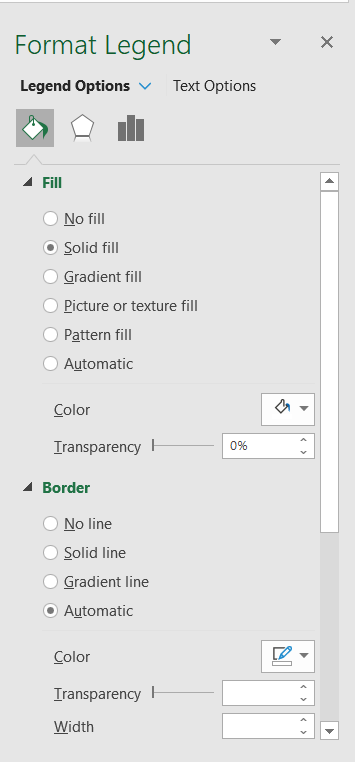
\includegraphics[width=0.2\linewidth]{images/format-legend.png}
	\caption{The format legend menu which can be used to change formatting of the chart.}%
	\label{fig:images_format-legend}
\end{figure}


\section{Analyzing Data}%
\label{sec:analyzing_data}

Now that you have your data plotted, it needs some analysis! Almost always, this will consist of doing some sort of fit.
This is a manual about spreadsheet programs, so we will focus less on the why and when of analyzing data, and more on some tools spreadsheet programs have for doing so. 

\subsection{Fit Lines}%
\label{sub:fit_lines}

A fit may be added to a plot using by clicking the ``Trendline'' box which shows up when you press the ``+'' button in the upper right-hand side of the chart.
This line will then appear on the plot, and you can optionally show the formula by checking a box that lives in the ``Format Trendline'' menu on the right. 

One of the drawbacks of using a fit line is that it is not clear how to get the uncertainty in the fit.
For example, suppose we are trying to find the velocity from a plot of position vs time.
Certainly the slope (assuming no acceleration) will be the velocity, but what will be the uncertainty in this value? While there are ways of finding it out, most spreadsheet programs provide a convenient function for accomplishing this.

\subsection{Linest}%
\label{sub:linest}

When dealing with linear data, the  \texttt{LINEST} function may be used to both fit the data, and get the uncertainties in the fit parameters.
Detailed documentation of the function can be found \href{https://support.microsoft.com/en-us/office/linest-function-84d7d0d9-6e50-4101-977a-fa7abf772b6d}{in the Excel manual}.
Here we give a brief description. 

The most confusing thing about this function is that is is an \textit{array formula}.
This means that, since it has multiple outputs (the fit parameters and their uncertainties), when Excel evaluates the formula, it replaces not just the value in the cell in which the \texttt{LINEST} is entered, but some of the surrounding cells. 

Lets take a look at how this works.
The function  \texttt{LINEST} takes 4 arguments.
The first is the range of y values that you want to look at, the second it the range of the x values that you want to look at.
Arguments 3 and 4 should be set to 1 (if you are interested in why, please see the page linked above).
Example usage is shown in Fig.~\ref{fig:linest}.

\begin{figure}
	\centering
	\begin{sheetpic}
		\etab[8]{A-F}
		\celtxt[c]{A}{1}{Time}
		\celtxt[c]{B}{1}{Position}
		\fillCol{A}{2}{8}{\row-1}{c}{}
		\calcCol{B}{2}{8}{A}{3 * \x + random()}{c}{}

		\celtxt[c]{D}{3}{3.1}
		\celtxt[c]{D}{4}{0.1}
		\celtxt[c]{D}{5}{0.41}
		\celtxt[c]{D}{6}{.1231}

		\celtxt[c]{E}{3}{.1231}
		\celtxt[c]{E}{4}{0.34}
		\celtxt[c]{E}{5}{0.1}
		\celtxt[c]{E}{6}{0.12}
		
		\annotateIm{(cellD-3.east)}{20}{2}{The slope of the fit}{}{}
		\annotateIm{(cellD-4.south)}{260}{3}{The uncertainty in the slope of the fit}{}{}
		\selecCell{D}{3}

		\annotateIm{(cellE-3.east)}{0}{3}{The y intercept of the fit}{}{}
		\annotateIm{(cellE-4.east)}{-20}{3}{The uncertainty in the y \\intercept of the fit}{align=center}{}
                \annotateIm{(cellD-3.north)}{80}{2}{ \texttt{=LINEST(B2:B8,A2:A8, 1,1)}}{}{}

	\end{sheetpic}
	\caption{Demonstrating the usage of LINEST. 
	Here we have entered the LINEST formula into cell D3, and see that it has filled the surrounding cells. }%
	\label{fig:linest}
\end{figure}

Note that the arguments to the \texttt{LINEST} function are separated by commas, and define some series of cells.
Either you can type them in as shown above (i.e.\texttt{FIRSTCELL:LASTCELL} syntax) or you can just click and drag to select each of the series.
Additionally, the function will populate several cells around where the formula is entered, so make sure that there is space around it.
Most of the outputted numbers are not useful to us, but the slope $m$ and $y$-intercept $b$, as well as their respective standard deviations (uncertainties) $\sigma_m$ and $\sigma_b$ are useful.
Their locations are pointed out in Fig.~\ref{fig:linest}.

As a final step in the data analysis, you can use the values outputted by \texttt{LINEST} to plot a line of best fit.
To do this, you just need to plot two points that fall on the line defined by the fit (recall that a line is uniquely defined by two points).
The points we will choose (for the purpose of the line being formatted correctly) will be $(x_1, y_1)$ and $(x_n, y_n)$, where $x_1$ and $x_n$ are the first and last of our $x$ data points, and $y_1$ and $y_n$ are calculated by the formula:
\[
y = mx + b
\]
with $m$ and $b$ gotten from \texttt{LINEST} as above.

We can calculate these values using formulas as discussed in section ~\ref{sec:formulas}, and then add the points to the plot as a data series as discussed in section ~\ref{sub:adding_data_to_a_chart}.

The only difference is that, in this case, we are not plotting data; we are plotting a fit curve.
We should style this as a solid line, as opposed to separate points.
To do this, click on the ``best fit points'' that you have plotted to bring up the ``Format Data Series'' menu on the right.
Click the paint bucket, and then you can change the style of the line and the marker to be how you want it.
A final plot is shown in Fig.~\ref{fig:images_finished-plot}.

\begin{figure}[htpb]
	\centering
	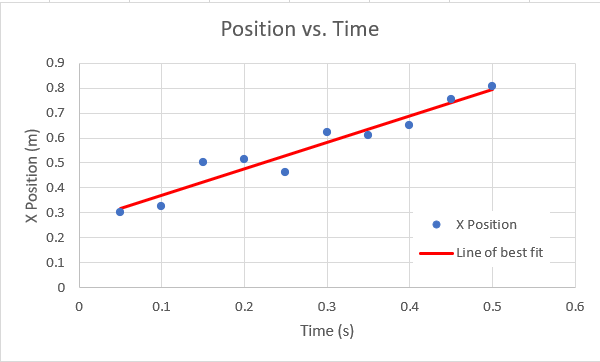
\includegraphics[width=0.8\linewidth]{images/finished-plot.png}
	\caption{The final plot that will go in your lab report}%
	\label{fig:images_finished-plot}
\end{figure}

This should be enough to get you started doing data analysis for labs in an introductory physics course.
If you get stuck on something, the first course of action is usually to try to google your problem -- it's likely someone has run into the same problem before.
If that doesn't solve it, do reach out to one of your peers or your TA; some struggle is helpful in the learning process, but it's not super helpful to keep banging your head against the wall on these kinds of minute technical problems. 

\end{document}
